\documentclass[11pt]{article}
\usepackage{epsfig}
\usepackage{amssymb}
\usepackage{fullpage}
\usepackage{color}
\usepackage{url}
\usepackage{natbib}
%\usepackage{emulateapj}
\usepackage{footnote}
\usepackage{deluxetable}
\usepackage{fancyvrb}

\newcommand{\aap}{A\&A}
\newcommand{\TODO}[1]{{\it \color{red} (#1)}}
\newcommand\codeHighlight[1]{\textcolor[rgb]{1,0,0}{\textbf{#1}}}

\begin{document}
\title{
DESI QSO Templates (v1.2)
}

\author{J. X. Prochaska (UCSC), J. Moustakas (Siena), S. Bailey
  (LBNL)}
\maketitle
\begin{center}

% Line below is modified automatically by svn, so don't edit it.
% Comment out the whole for final document
% (I first did : svn propset svn:keywords 'Id Author Date Rev' qso-templates.tex)
{\small SVN $ $Rev: 2833 $ $, $ $Date: 2014-12-22 07:28:33 -0800 (Mon, 22 Dec 2014) $ $, $ $Author: profx $ $ }
\end{center}

\abstract{ This technote documents the construction of the preliminary
  (v1.1) QSO templates for DESI.  It also describes how one may 
  generate new, random sets of QSO templates (on-the-fly) in desisim. }

\section{Introduction}

DESI will obtain high-resolution, observed-frame optical spectroscopy
of four broad classes of objects: quasars (QSOs), emission-line
galaxies (ELGs), luminous red galaxies (LRGs), and stars.  Reliable
spectral templates are critical for several key aspects of the
Project, including spectral simulations (constructing mock datasets),
optimization of targeting strategies, redshift fitting, spectral
classification, and other applications.

The general requirements on the spectral templates for all four
classes of objects are: (1) broad coverage of physical parameter
space; (2) wide wavelength coverage (minimum rest-frame
$\approx0.15-1~\mu$m spectral coverage); (3) high spectral
resolution (at least $\mathcal{R}\approx4500$); and (4) high
spectrophotometric fidelity.

This document describes the construction of the \emph{preliminary} QSO
templates for DESI.  These templates are generated from a PCA analysis
of SDSS/DR7 quasar spectra ($0.4<z<2$) and BOSS/DR10 quasar spectra
($z=2-4$), as described in Section~\ref{sec:sdssboss}.  We generated
500 templates per $\Delta z = 0.2$ interval from $z=0.4 - 4$,
uniformly sampling in redshift in each bin.  Further details on the
spectra are provided in Section~\ref{sec:templ}.

\section{SDSS/BOSS Spectroscopy}\label{sec:sdssboss}

\subsection{PCA Analysis}

The BOSS team has previously generated PCA eigenvectors from a sample
of approximately 450 quasars using the standard {\tt IDLSPEC2D}
algorithms.  The four eigenvectors are recorded in the file {\tt
  spEigenQSO-55732.fits}.  These spectra cover the rest-frame
450.2-10400\AA\ spectral range with a constant logarithmic dispersion
of $10^{-4}$~log$_{10}$~\AA{} (approximately $70$~km~s$^{-1}$ per
pixel).  We show these four eigenspectra in Figure~\ref{fig:eigen}.
One appreciates that most of the flux is in {\tt Eigen0} (as
expected), and that the eigenvectors are not physical representations
of actual quasars.  Nevertheless, we find these provide an excellent
basis for the observed spectra.

These eignevectors were fitted to observed SDSS and BOSS spectra using
standard least-squares (inverse variance weighted) fitting.  In this
analysis we do not use the spectral masks developed for BOSS, nor do
we develop our own masks (e.g.\ for known, bright sky lines).
However, we examined several tens of the fits by-eye to assess
performance and found generally good results.

\begin{figure}[h!]
  \vskip -0.1in
\begin{center}
  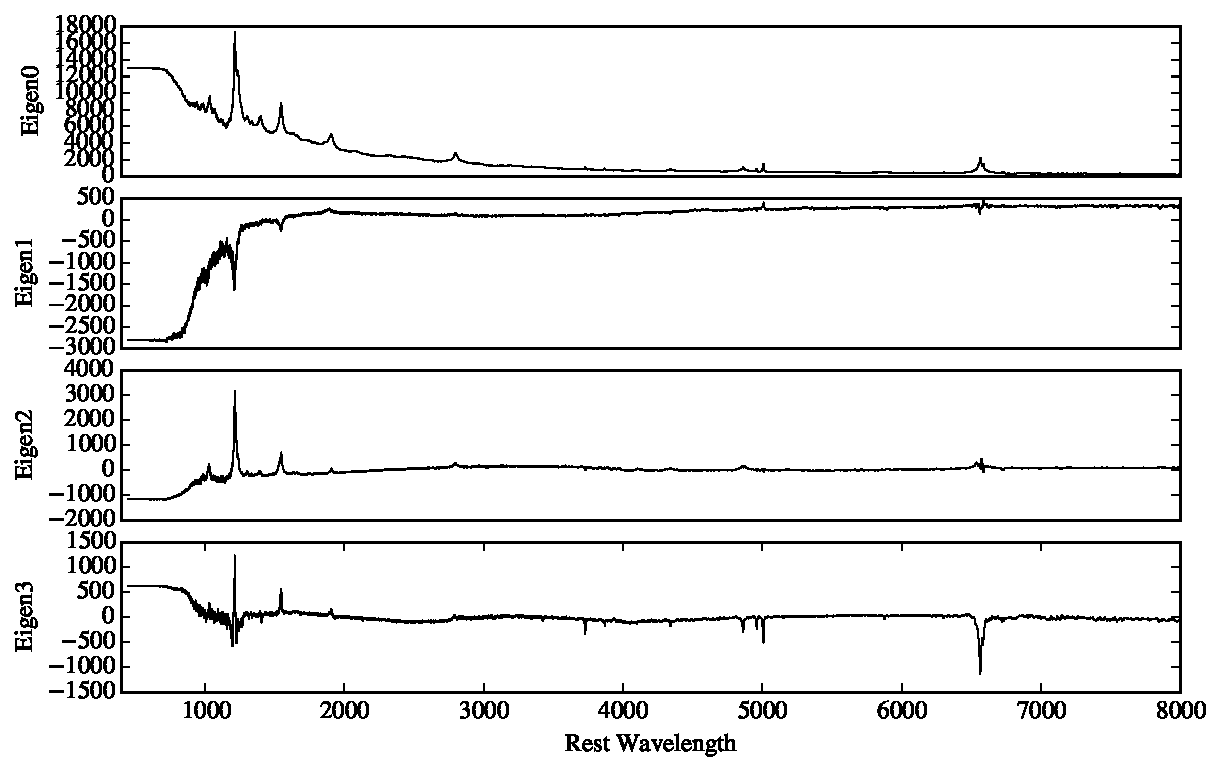
\includegraphics[width=5in]{figures/fig_boss_eigen.pdf}
\end{center}
 \vskip -0.20in
  \caption{\footnotesize 
    PCA eigenvectors drawn from the BOSS spectral package,
    specifically file spEigenQSO-55732.fits.  These span from $\approx
    450-10,400$\AA\ in the rest-frame.
 }\label{fig:eigen}
\vskip -0.1in
\end{figure}

\subsection{SDSS DR7}\label{sec:sdss}

We analyzed approximately 100,000 quasars drawn from the SDSS/DR7
quasar catalog, with spectra from the {\tt 1d\_26} extraction.  In our
adopted bins of $\Delta z = 0.2$, there are many thousands of spectra
per bin.  Unlike DESI (and BOSS), these data have a starting
wavelength of $\approx 3800$\AA.  Therefore, in the subsequent
analysis we assume a modest extrapolation of the solutions to bluer
wavelengths.  The models, however, appear well-behaved.

Figure~\ref{fig:sdss_pca} compares the distributions of the four PCA
coefficients derived for all of the SDSS spectra.  The variation in
the values is small, consistent with the small variation in quasar
spectral energy distributions (SEDs). Most of the variation in {\tt
  PCA0} derives from variations in the observed flux of these sources.
One does identify modest correlation between several pairs of the PCA
components (e.g. {\tt PCA1} vs.\ {\tt PCA3}).  When generating the
templates, however, we consider the PCA components independently. 

\begin{figure}[h!]
  \vskip -0.1in
\begin{center}
  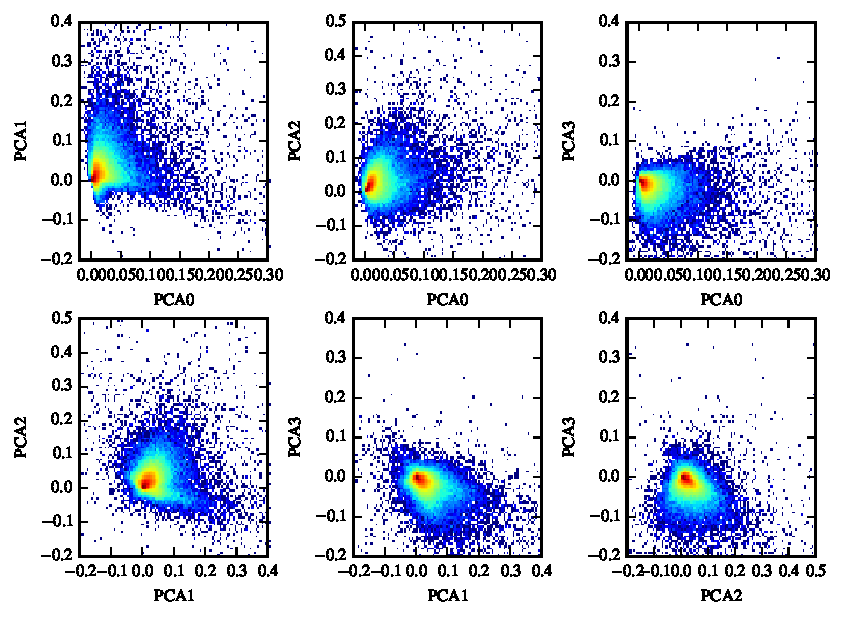
\includegraphics[width=5in]{figures/fig_sdss_pca.pdf}
\end{center}
 \vskip -0.20in
  \caption{\footnotesize PCA coefficients derived from $\approx
    100,000$ SDSS/DR7 quasars.  Color (red to blue) illustrates the
    number of sources at the plotted values.  Most of the variation in
    PCA0 derives from variations in the observed flux of these
    sources.  One does identify modest correlation between several
    pairs of the PCA components (e.g. PCA1 vs.\ PCA3).
  }\label{fig:sdss_pca}
\vskip -0.1in
\end{figure}

\subsection{BOSS/DR10}

We have analyzed approximately 100,000 quasars from BOSS/DR10, which
were used to study the Ly$\alpha$ forest by K.G. Lee ({\tt v2.1} of
his catalogs).  These quasars are almost exclusively at $z>2$, and as
with all BOSS spectra span the $\approx 3600-10,000$~\AA{} spectral
range. 

As in Section~\ref{sec:sdss} when analyzing the SDSS data, we derive
PCA coefficients from the BOSS spectra and find small variation in the
values.  Figure~\ref{fig:boss_pca_vs_i} shows the dependence of the
PCA values on $i$-band magnitude (which also correlates with
redshift).  As expected, {\tt PCA0}n shows the greatest correlation
with $i$-band magnitude.  We speculate that the dispersion in the PCA
values decreases with increasing magnitude owing to the poorer S/N of
the spectra.

\begin{figure}[h!]
  \vskip -0.1in
\begin{center}
  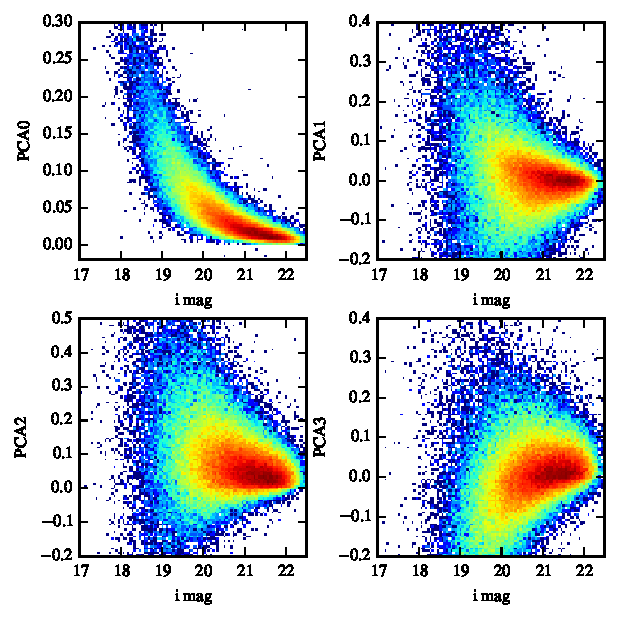
\includegraphics[width=5in]{figures/fig_boss_imag_vs_pca.pdf}
\end{center}
 \vskip -0.20in
  \caption{\footnotesize PCA coefficients of the BOSS/DR10 Ly$\alpha$
    sample as a function of $i$ magnitude.  As expected, {\tt PCA0}
    shows the greatest variation with observed quasar flux.  We
    suspect that the reduced dispersion in the PCA values with
    increasing magnitude is due to poorer S/N of those spectra, not a
    physical effect.  }\label{fig:boss_pca_vs_i}
\vskip -0.1in
\end{figure}


\section{QSO Templates}\label{sec:templ}

From the measured PCA values of the SDSS and BOSS samples, we proceed
to construct a set of 9,000 quasar templates as follows.  Note that we
use the SDSS models to construct templates at $z<2$ and the BOSS
spectra otherwise.

Stepping on a redshift interval of $\Delta z = 0.2$ and starting at
$z=0.2$, we generate {\tt N\_perz=500} quasar templates per $\Delta z$
interval to $z=4$.  For
these 500 templates we adopt the following approach:

\begin{enumerate}
\item Draw $z$ uniformly between the bounds of the interval.
\item For {\tt PCA0}, calculate the interval encompassing 95\%\ of the
  measured values.  These generally do not follow a Gaussian
  distribution.
\item For {\tt PCA1}, calculate the standard deviation.
\item Sample each PCA distribution uniformly over the 95\% confidence
  interval (i.e.\ $2 \sigma$ for {\tt PCA1-3}).
\item Generate a template from these random PCA values and the
  eigenvectors. 
\item Discard the template if the flux is negative in the rest-frame
  interval $900-5000$\AA.  This occurs approximately $5\%-10$\%\ of
  the time.
\item If $z \ge 2.4$, attenuate the flux shortward of $911.76$\AA\ in
  the rest-frame by a statistical estimate of the Lyman continuum (see
  below).
\item Convert to the observer frame and interpolate on a $\log_{10}$
  wavelength grid with $10$~km~s$^{-1}$ pixels starting at
  $3500$\AA\ and extending to $10,000$~\AA.
\end{enumerate}

For the Lyman continuum attenuation, we adopt the mean-free-path
$\lambda_{\rm MFP}$ estimates from Worseck et~al. (2014).
%\citet{worseck14a}
We then calculate the physical distance from the source $r_{\rm phys}$
with a standard $\Lambda$CDM cosmology ($\Omega_m = 0.3$), and then
attenuate the flux by $\exp(-r_{\rm phys} / \lambda_{\rm MFP})$. 

Figure~\ref{fig:gallery} shows a set of example templates.
The flux are in units of erg/s/cm$^2$/\AA\ and 
normalized to $10^{-17}$.

\begin{figure}[h!]
  \vskip -0.1in
\begin{center}
  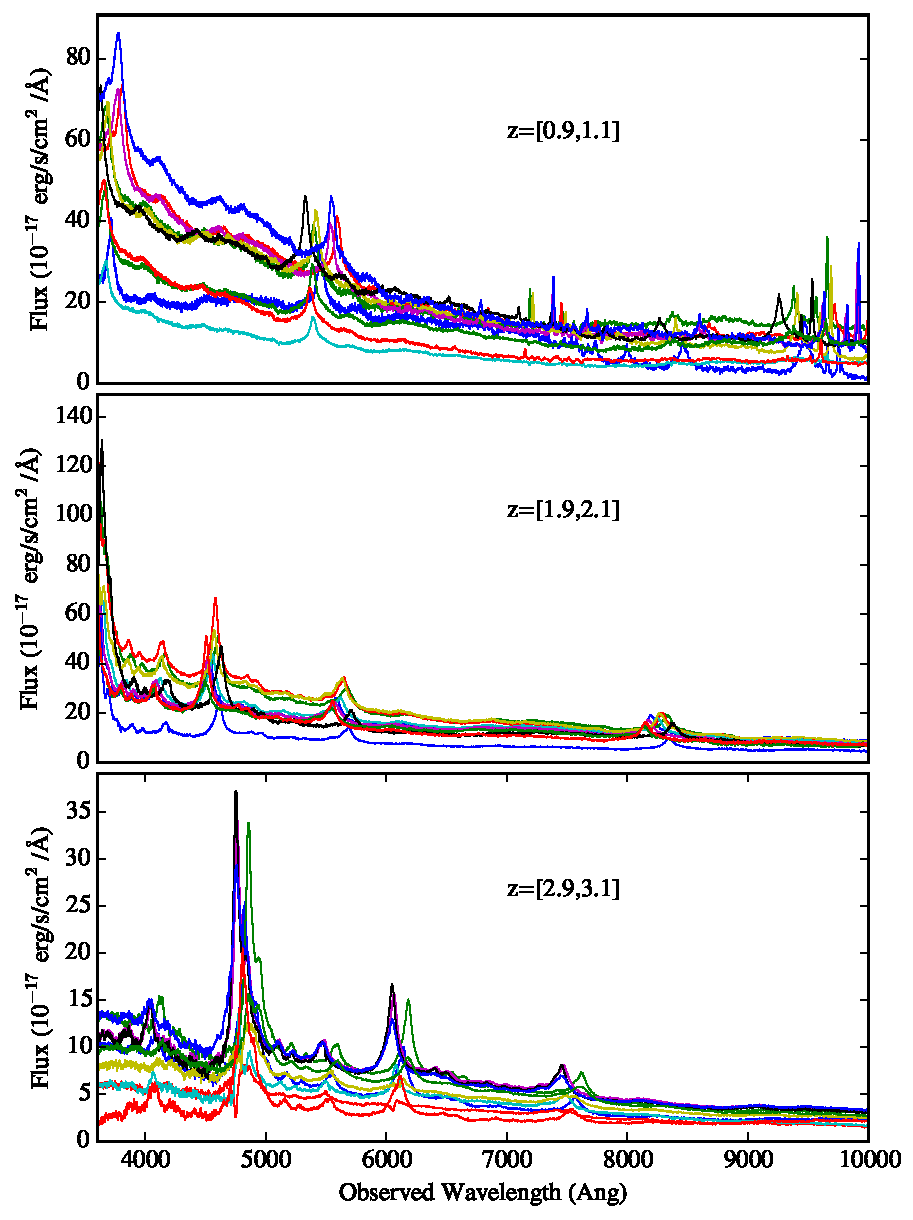
\includegraphics[width=5in]{figures/fig_desi_template_gallery.pdf}
\end{center}
 \vskip -0.20in
  \caption{\footnotesize Gallery of DESI quasar templates at $z \sim
    [1,2,3]$.  One observes a diversity of emission strengths,
    spectral slopes and IGM opacity.
}\label{fig:gallery}
\vskip -0.1in
\end{figure}


\section{Ancillary Information}

All of the codes for this analysis are in the DESI github repository
under py/qso\_template.  Here are the primary modules:

\begin{itemize}
\item {\tt fit\_boss\_qsos.py} -- Module for fitting the eigenvectors
  to the SDSS and BOSS spectra
\item {\tt run\_qso\_fits.py} -- Module for (simple) parallelization
  of the fitting
\item {\tt desi\_qso\_templ.py} -- Module for generating the DESI
  quasar templates
\item {\tt boss\_qsos\_figs.py} -- Module for generating figures from
  the various outputs.
\end{itemize}

Some of these codes draw on modules in the {\tt xastropy} and {\tt
  astropy} packages.

\vskip 0.2in


The templates can be found on NERSC in {\tt
  \$\{DESI\_ROOT\}/spectro/templates/qso\_templates/VERSION}, where
{\tt VERSION} is the template version number (currently v1.1).  The
template file itself, {\tt qso\_templates\_v1.1.fits} is a binary FITS
table with two extensions:

\begin{enumerate}
\item Extension~0: An [{\sc npixel}]$\times$[{\sc ntemplate}] flux
  array which contains {\sc ntemplate} spectra, each {\sc npixel}
  pixels long.
\item Extension~1: An [{\sc ntemplate}] data structure with the
  following metadata:
\begin{itemize}
\item{.{\sc TEMPLATEID} - unique template ID number (zero-indexed)}
\item{.{\sc Z} - redshift of the source}
\end{itemize}
\end{enumerate}

\section{Generating New Templates}\label{sec:new_templ}

Users may wish to generate templates beyond the v1.1 set.
The code has now been refactored to allow such activity.
Presently, the user generates a new FITS file containing 
the new set of templates.  The code also returns the specta
as simple numpy arrays.  

\begin{Verbatim}[commandchars=\\\{\}]
final_wave, final_spec, final_z = desi_qso_templates(outfil='test_random_set.fits', 
   N_perz=100, seed=12345)
\end{Verbatim}

The data necessary to run this
bit of code is currently here at NERSC: \\
{\tt /project/projectdirs/desi/spectro/templates/basis\_templates/v2.0/qso\_templates\_v2.0.fits}

\section{Future Improvements}\label{sec:future}

Future improvements to these templates may include (in no particular
order): 

\begin{itemize}
\item Masking of pixels in the PCA analysis.
\item Generate eigenvectors from the full and combined BOSS/SDSS datasets.
\item Apply the analysis to flux-corrected BOSS spectra.
\item Implementation of a stochastic Ly$\alpha$ forest.
\item Account for correlation between the PCA coefficients. 
\item Include BALs and other `unusual' quasars.
\end{itemize}

%\bibliographystyle{apj}
%\bibliography{/Users/ioannis/bibdesk/ioannis}
%\documentclass[11pt]{article}
\usepackage{epsfig}
\usepackage{amssymb}
\usepackage{fullpage}
\usepackage{color}
\usepackage{url}
\usepackage{natbib}
%\usepackage{emulateapj}
\usepackage{footnote}
\usepackage{deluxetable}
\usepackage{fancyvrb}

\newcommand{\aap}{A\&A}
\newcommand{\TODO}[1]{{\it \color{red} (#1)}}
\newcommand\codeHighlight[1]{\textcolor[rgb]{1,0,0}{\textbf{#1}}}

\begin{document}
\title{
DESI QSO Templates (v1.2)
}

\author{J. X. Prochaska (UCSC), J. Moustakas (Siena), S. Bailey
  (LBNL)}
\maketitle
\begin{center}

% Line below is modified automatically by svn, so don't edit it.
% Comment out the whole for final document
% (I first did : svn propset svn:keywords 'Id Author Date Rev' qso-templates.tex)
{\small SVN $ $Rev: 2833 $ $, $ $Date: 2014-12-22 07:28:33 -0800 (Mon, 22 Dec 2014) $ $, $ $Author: profx $ $ }
\end{center}

\abstract{ This technote documents the construction of the preliminary
  (v1.1) QSO templates for DESI.  It also describes how one may 
  generate new, random sets of QSO templates (on-the-fly) in desisim. }

\section{Introduction}

DESI will obtain high-resolution, observed-frame optical spectroscopy
of four broad classes of objects: quasars (QSOs), emission-line
galaxies (ELGs), luminous red galaxies (LRGs), and stars.  Reliable
spectral templates are critical for several key aspects of the
Project, including spectral simulations (constructing mock datasets),
optimization of targeting strategies, redshift fitting, spectral
classification, and other applications.

The general requirements on the spectral templates for all four
classes of objects are: (1) broad coverage of physical parameter
space; (2) wide wavelength coverage (minimum rest-frame
$\approx0.15-1~\mu$m spectral coverage); (3) high spectral
resolution (at least $\mathcal{R}\approx4500$); and (4) high
spectrophotometric fidelity.

This document describes the construction of the \emph{preliminary} QSO
templates for DESI.  These templates are generated from a PCA analysis
of SDSS/DR7 quasar spectra ($0.4<z<2$) and BOSS/DR10 quasar spectra
($z=2-4$), as described in Section~\ref{sec:sdssboss}.  We generated
500 templates per $\Delta z = 0.2$ interval from $z=0.4 - 4$,
uniformly sampling in redshift in each bin.  Further details on the
spectra are provided in Section~\ref{sec:templ}.

\section{SDSS/BOSS Spectroscopy}\label{sec:sdssboss}

\subsection{PCA Analysis}

The BOSS team has previously generated PCA eigenvectors from a sample
of approximately 450 quasars using the standard {\tt IDLSPEC2D}
algorithms.  The four eigenvectors are recorded in the file {\tt
  spEigenQSO-55732.fits}.  These spectra cover the rest-frame
450.2-10400\AA\ spectral range with a constant logarithmic dispersion
of $10^{-4}$~log$_{10}$~\AA{} (approximately $70$~km~s$^{-1}$ per
pixel).  We show these four eigenspectra in Figure~\ref{fig:eigen}.
One appreciates that most of the flux is in {\tt Eigen0} (as
expected), and that the eigenvectors are not physical representations
of actual quasars.  Nevertheless, we find these provide an excellent
basis for the observed spectra.

These eignevectors were fitted to observed SDSS and BOSS spectra using
standard least-squares (inverse variance weighted) fitting.  In this
analysis we do not use the spectral masks developed for BOSS, nor do
we develop our own masks (e.g.\ for known, bright sky lines).
However, we examined several tens of the fits by-eye to assess
performance and found generally good results.

\begin{figure}[h!]
  \vskip -0.1in
\begin{center}
  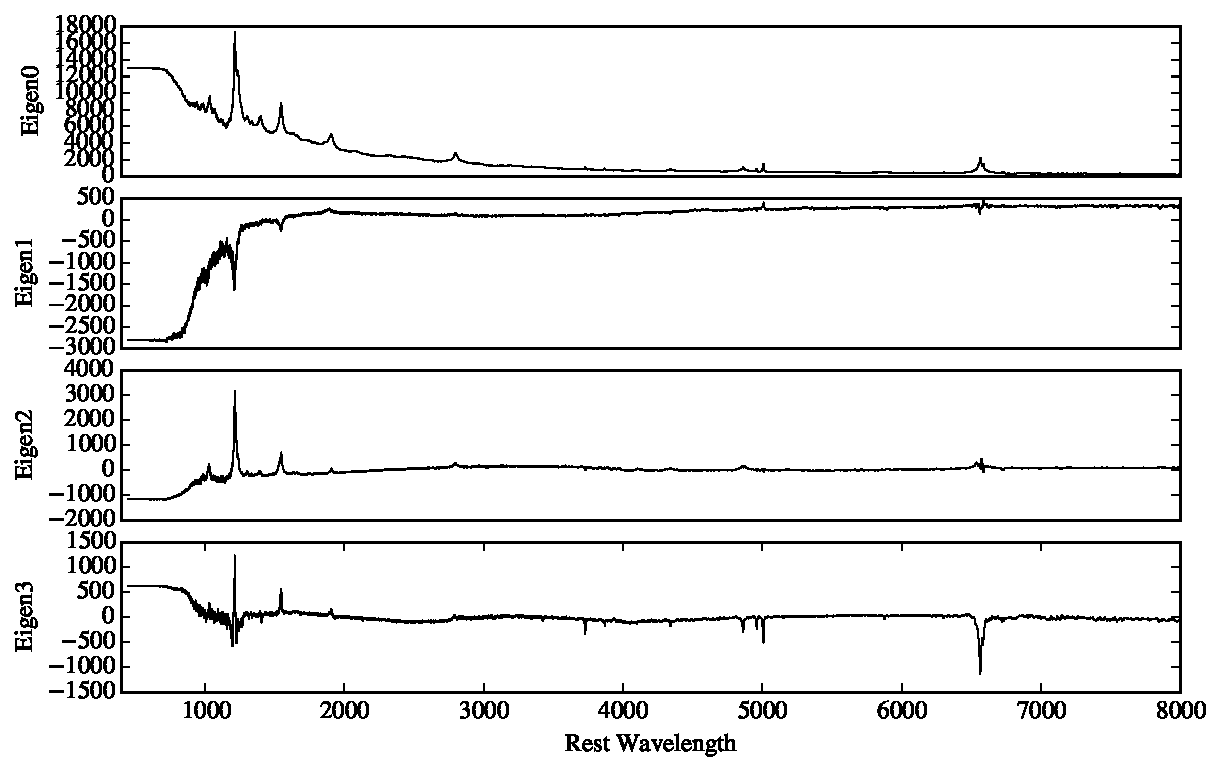
\includegraphics[width=5in]{figures/fig_boss_eigen.pdf}
\end{center}
 \vskip -0.20in
  \caption{\footnotesize 
    PCA eigenvectors drawn from the BOSS spectral package,
    specifically file spEigenQSO-55732.fits.  These span from $\approx
    450-10,400$\AA\ in the rest-frame.
 }\label{fig:eigen}
\vskip -0.1in
\end{figure}

\subsection{SDSS DR7}\label{sec:sdss}

We analyzed approximately 100,000 quasars drawn from the SDSS/DR7
quasar catalog, with spectra from the {\tt 1d\_26} extraction.  In our
adopted bins of $\Delta z = 0.2$, there are many thousands of spectra
per bin.  Unlike DESI (and BOSS), these data have a starting
wavelength of $\approx 3800$\AA.  Therefore, in the subsequent
analysis we assume a modest extrapolation of the solutions to bluer
wavelengths.  The models, however, appear well-behaved.

Figure~\ref{fig:sdss_pca} compares the distributions of the four PCA
coefficients derived for all of the SDSS spectra.  The variation in
the values is small, consistent with the small variation in quasar
spectral energy distributions (SEDs). Most of the variation in {\tt
  PCA0} derives from variations in the observed flux of these sources.
One does identify modest correlation between several pairs of the PCA
components (e.g. {\tt PCA1} vs.\ {\tt PCA3}).  When generating the
templates, however, we consider the PCA components independently. 

\begin{figure}[h!]
  \vskip -0.1in
\begin{center}
  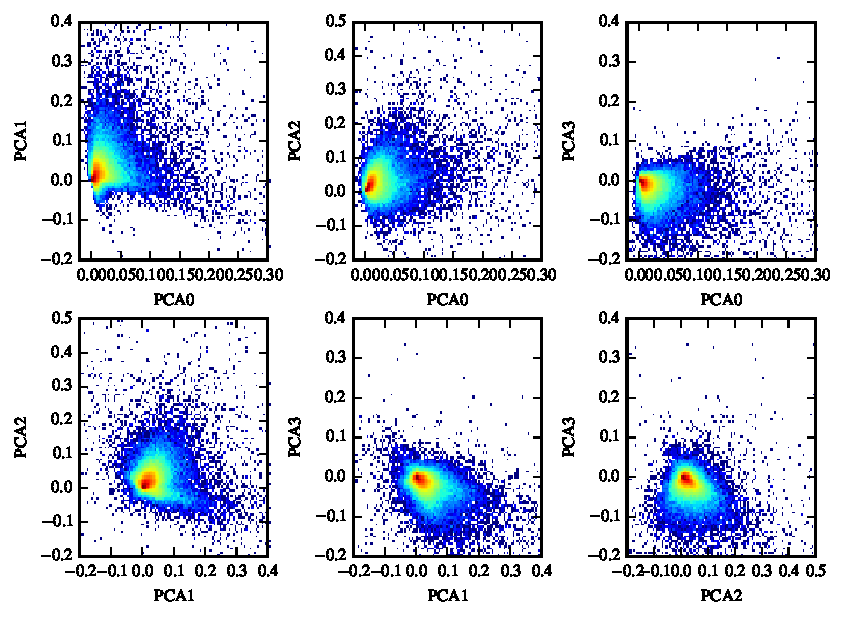
\includegraphics[width=5in]{figures/fig_sdss_pca.pdf}
\end{center}
 \vskip -0.20in
  \caption{\footnotesize PCA coefficients derived from $\approx
    100,000$ SDSS/DR7 quasars.  Color (red to blue) illustrates the
    number of sources at the plotted values.  Most of the variation in
    PCA0 derives from variations in the observed flux of these
    sources.  One does identify modest correlation between several
    pairs of the PCA components (e.g. PCA1 vs.\ PCA3).
  }\label{fig:sdss_pca}
\vskip -0.1in
\end{figure}

\subsection{BOSS/DR10}

We have analyzed approximately 100,000 quasars from BOSS/DR10, which
were used to study the Ly$\alpha$ forest by K.G. Lee ({\tt v2.1} of
his catalogs).  These quasars are almost exclusively at $z>2$, and as
with all BOSS spectra span the $\approx 3600-10,000$~\AA{} spectral
range. 

As in Section~\ref{sec:sdss} when analyzing the SDSS data, we derive
PCA coefficients from the BOSS spectra and find small variation in the
values.  Figure~\ref{fig:boss_pca_vs_i} shows the dependence of the
PCA values on $i$-band magnitude (which also correlates with
redshift).  As expected, {\tt PCA0}n shows the greatest correlation
with $i$-band magnitude.  We speculate that the dispersion in the PCA
values decreases with increasing magnitude owing to the poorer S/N of
the spectra.

\begin{figure}[h!]
  \vskip -0.1in
\begin{center}
  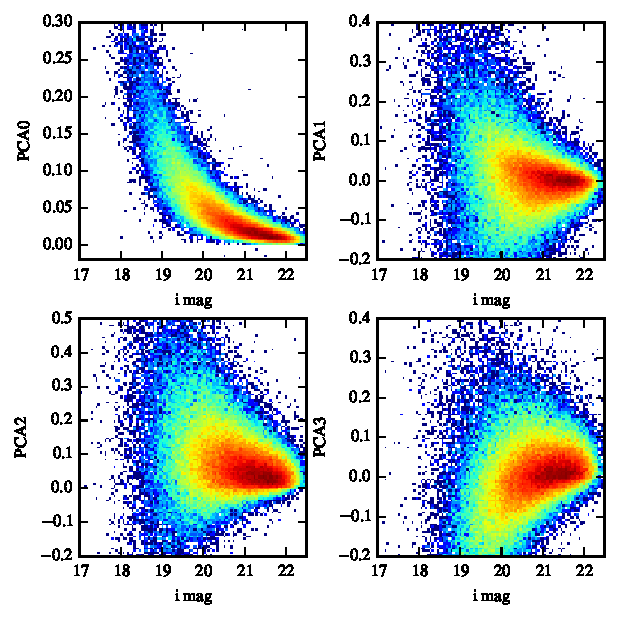
\includegraphics[width=5in]{figures/fig_boss_imag_vs_pca.pdf}
\end{center}
 \vskip -0.20in
  \caption{\footnotesize PCA coefficients of the BOSS/DR10 Ly$\alpha$
    sample as a function of $i$ magnitude.  As expected, {\tt PCA0}
    shows the greatest variation with observed quasar flux.  We
    suspect that the reduced dispersion in the PCA values with
    increasing magnitude is due to poorer S/N of those spectra, not a
    physical effect.  }\label{fig:boss_pca_vs_i}
\vskip -0.1in
\end{figure}


\section{QSO Templates}\label{sec:templ}

From the measured PCA values of the SDSS and BOSS samples, we proceed
to construct a set of 9,000 quasar templates as follows.  Note that we
use the SDSS models to construct templates at $z<2$ and the BOSS
spectra otherwise.

Stepping on a redshift interval of $\Delta z = 0.2$ and starting at
$z=0.2$, we generate {\tt N\_perz=500} quasar templates per $\Delta z$
interval to $z=4$.  For
these 500 templates we adopt the following approach:

\begin{enumerate}
\item Draw $z$ uniformly between the bounds of the interval.
\item For {\tt PCA0}, calculate the interval encompassing 95\%\ of the
  measured values.  These generally do not follow a Gaussian
  distribution.
\item For {\tt PCA1}, calculate the standard deviation.
\item Sample each PCA distribution uniformly over the 95\% confidence
  interval (i.e.\ $2 \sigma$ for {\tt PCA1-3}).
\item Generate a template from these random PCA values and the
  eigenvectors. 
\item Discard the template if the flux is negative in the rest-frame
  interval $900-5000$\AA.  This occurs approximately $5\%-10$\%\ of
  the time.
\item If $z \ge 2.4$, attenuate the flux shortward of $911.76$\AA\ in
  the rest-frame by a statistical estimate of the Lyman continuum (see
  below).
\item Convert to the observer frame and interpolate on a $\log_{10}$
  wavelength grid with $10$~km~s$^{-1}$ pixels starting at
  $3500$\AA\ and extending to $10,000$~\AA.
\end{enumerate}

For the Lyman continuum attenuation, we adopt the mean-free-path
$\lambda_{\rm MFP}$ estimates from Worseck et~al. (2014).
%\citet{worseck14a}
We then calculate the physical distance from the source $r_{\rm phys}$
with a standard $\Lambda$CDM cosmology ($\Omega_m = 0.3$), and then
attenuate the flux by $\exp(-r_{\rm phys} / \lambda_{\rm MFP})$. 

Figure~\ref{fig:gallery} shows a set of example templates.
The flux are in units of erg/s/cm$^2$/\AA\ and 
normalized to $10^{-17}$.

\begin{figure}[h!]
  \vskip -0.1in
\begin{center}
  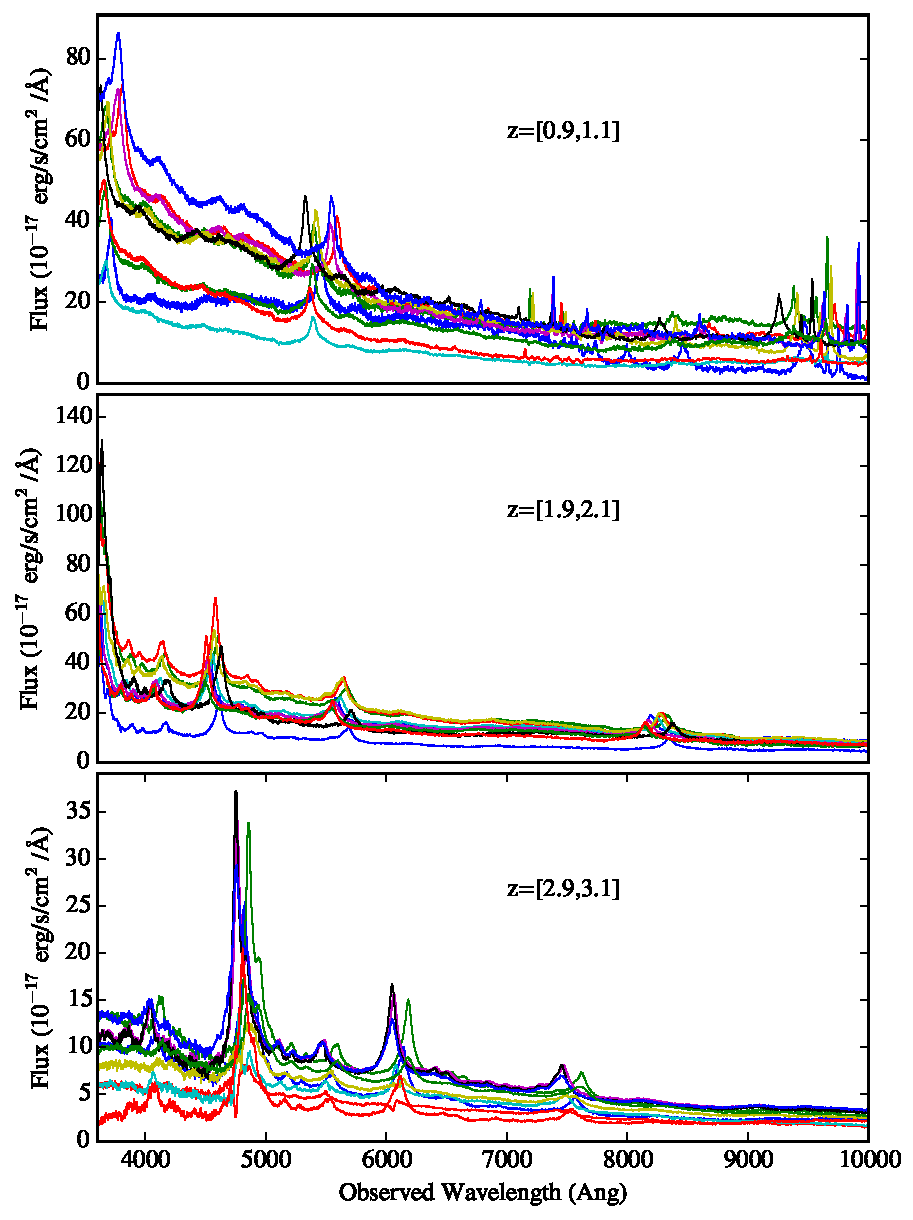
\includegraphics[width=5in]{figures/fig_desi_template_gallery.pdf}
\end{center}
 \vskip -0.20in
  \caption{\footnotesize Gallery of DESI quasar templates at $z \sim
    [1,2,3]$.  One observes a diversity of emission strengths,
    spectral slopes and IGM opacity.
}\label{fig:gallery}
\vskip -0.1in
\end{figure}


\section{Ancillary Information}

All of the codes for this analysis are in the DESI github repository
under py/qso\_template.  Here are the primary modules:

\begin{itemize}
\item {\tt fit\_boss\_qsos.py} -- Module for fitting the eigenvectors
  to the SDSS and BOSS spectra
\item {\tt run\_qso\_fits.py} -- Module for (simple) parallelization
  of the fitting
\item {\tt desi\_qso\_templ.py} -- Module for generating the DESI
  quasar templates
\item {\tt boss\_qsos\_figs.py} -- Module for generating figures from
  the various outputs.
\end{itemize}

Some of these codes draw on modules in the {\tt xastropy} and {\tt
  astropy} packages.

\vskip 0.2in


The templates can be found on NERSC in {\tt
  \$\{DESI\_ROOT\}/spectro/templates/qso\_templates/VERSION}, where
{\tt VERSION} is the template version number (currently v1.1).  The
template file itself, {\tt qso\_templates\_v1.1.fits} is a binary FITS
table with two extensions:

\begin{enumerate}
\item Extension~0: An [{\sc npixel}]$\times$[{\sc ntemplate}] flux
  array which contains {\sc ntemplate} spectra, each {\sc npixel}
  pixels long.
\item Extension~1: An [{\sc ntemplate}] data structure with the
  following metadata:
\begin{itemize}
\item{.{\sc TEMPLATEID} - unique template ID number (zero-indexed)}
\item{.{\sc Z} - redshift of the source}
\end{itemize}
\end{enumerate}

\section{Generating New Templates}\label{sec:new_templ}

Users may wish to generate templates beyond the v1.1 set.
The code has now been refactored to allow such activity.
Presently, the user generates a new FITS file containing 
the new set of templates.  The code also returns the specta
as simple numpy arrays.  

\begin{Verbatim}[commandchars=\\\{\}]
final_wave, final_spec, final_z = desi_qso_templates(outfil='test_random_set.fits', 
   N_perz=100, seed=12345)
\end{Verbatim}

The data necessary to run this
bit of code is currently here at NERSC: \\
{\tt /project/projectdirs/desi/spectro/templates/basis\_templates/v2.0/qso\_templates\_v2.0.fits}

\section{Future Improvements}\label{sec:future}

Future improvements to these templates may include (in no particular
order): 

\begin{itemize}
\item Masking of pixels in the PCA analysis.
\item Generate eigenvectors from the full and combined BOSS/SDSS datasets.
\item Apply the analysis to flux-corrected BOSS spectra.
\item Implementation of a stochastic Ly$\alpha$ forest.
\item Account for correlation between the PCA coefficients. 
\item Include BALs and other `unusual' quasars.
\end{itemize}

%\bibliographystyle{apj}
%\bibliography{/Users/ioannis/bibdesk/ioannis}
%\documentclass[11pt]{article}
\usepackage{epsfig}
\usepackage{amssymb}
\usepackage{fullpage}
\usepackage{color}
\usepackage{url}
\usepackage{natbib}
%\usepackage{emulateapj}
\usepackage{footnote}
\usepackage{deluxetable}
\usepackage{fancyvrb}

\newcommand{\aap}{A\&A}
\newcommand{\TODO}[1]{{\it \color{red} (#1)}}
\newcommand\codeHighlight[1]{\textcolor[rgb]{1,0,0}{\textbf{#1}}}

\begin{document}
\title{
DESI QSO Templates (v1.2)
}

\author{J. X. Prochaska (UCSC), J. Moustakas (Siena), S. Bailey
  (LBNL)}
\maketitle
\begin{center}

% Line below is modified automatically by svn, so don't edit it.
% Comment out the whole for final document
% (I first did : svn propset svn:keywords 'Id Author Date Rev' qso-templates.tex)
{\small SVN $ $Rev: 2833 $ $, $ $Date: 2014-12-22 07:28:33 -0800 (Mon, 22 Dec 2014) $ $, $ $Author: profx $ $ }
\end{center}

\abstract{ This technote documents the construction of the preliminary
  (v1.1) QSO templates for DESI.  It also describes how one may 
  generate new, random sets of QSO templates (on-the-fly) in desisim. }

\section{Introduction}

DESI will obtain high-resolution, observed-frame optical spectroscopy
of four broad classes of objects: quasars (QSOs), emission-line
galaxies (ELGs), luminous red galaxies (LRGs), and stars.  Reliable
spectral templates are critical for several key aspects of the
Project, including spectral simulations (constructing mock datasets),
optimization of targeting strategies, redshift fitting, spectral
classification, and other applications.

The general requirements on the spectral templates for all four
classes of objects are: (1) broad coverage of physical parameter
space; (2) wide wavelength coverage (minimum rest-frame
$\approx0.15-1~\mu$m spectral coverage); (3) high spectral
resolution (at least $\mathcal{R}\approx4500$); and (4) high
spectrophotometric fidelity.

This document describes the construction of the \emph{preliminary} QSO
templates for DESI.  These templates are generated from a PCA analysis
of SDSS/DR7 quasar spectra ($0.4<z<2$) and BOSS/DR10 quasar spectra
($z=2-4$), as described in Section~\ref{sec:sdssboss}.  We generated
500 templates per $\Delta z = 0.2$ interval from $z=0.4 - 4$,
uniformly sampling in redshift in each bin.  Further details on the
spectra are provided in Section~\ref{sec:templ}.

\section{SDSS/BOSS Spectroscopy}\label{sec:sdssboss}

\subsection{PCA Analysis}

The BOSS team has previously generated PCA eigenvectors from a sample
of approximately 450 quasars using the standard {\tt IDLSPEC2D}
algorithms.  The four eigenvectors are recorded in the file {\tt
  spEigenQSO-55732.fits}.  These spectra cover the rest-frame
450.2-10400\AA\ spectral range with a constant logarithmic dispersion
of $10^{-4}$~log$_{10}$~\AA{} (approximately $70$~km~s$^{-1}$ per
pixel).  We show these four eigenspectra in Figure~\ref{fig:eigen}.
One appreciates that most of the flux is in {\tt Eigen0} (as
expected), and that the eigenvectors are not physical representations
of actual quasars.  Nevertheless, we find these provide an excellent
basis for the observed spectra.

These eignevectors were fitted to observed SDSS and BOSS spectra using
standard least-squares (inverse variance weighted) fitting.  In this
analysis we do not use the spectral masks developed for BOSS, nor do
we develop our own masks (e.g.\ for known, bright sky lines).
However, we examined several tens of the fits by-eye to assess
performance and found generally good results.

\begin{figure}[h!]
  \vskip -0.1in
\begin{center}
  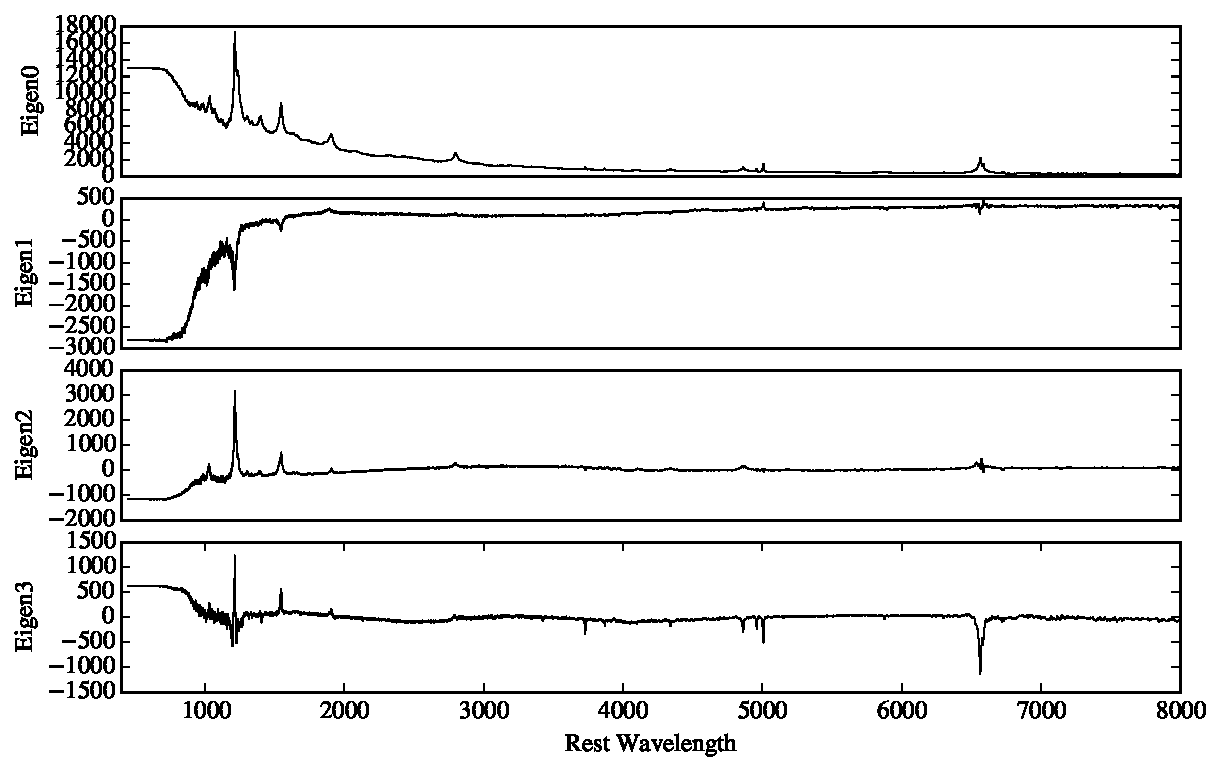
\includegraphics[width=5in]{figures/fig_boss_eigen.pdf}
\end{center}
 \vskip -0.20in
  \caption{\footnotesize 
    PCA eigenvectors drawn from the BOSS spectral package,
    specifically file spEigenQSO-55732.fits.  These span from $\approx
    450-10,400$\AA\ in the rest-frame.
 }\label{fig:eigen}
\vskip -0.1in
\end{figure}

\subsection{SDSS DR7}\label{sec:sdss}

We analyzed approximately 100,000 quasars drawn from the SDSS/DR7
quasar catalog, with spectra from the {\tt 1d\_26} extraction.  In our
adopted bins of $\Delta z = 0.2$, there are many thousands of spectra
per bin.  Unlike DESI (and BOSS), these data have a starting
wavelength of $\approx 3800$\AA.  Therefore, in the subsequent
analysis we assume a modest extrapolation of the solutions to bluer
wavelengths.  The models, however, appear well-behaved.

Figure~\ref{fig:sdss_pca} compares the distributions of the four PCA
coefficients derived for all of the SDSS spectra.  The variation in
the values is small, consistent with the small variation in quasar
spectral energy distributions (SEDs). Most of the variation in {\tt
  PCA0} derives from variations in the observed flux of these sources.
One does identify modest correlation between several pairs of the PCA
components (e.g. {\tt PCA1} vs.\ {\tt PCA3}).  When generating the
templates, however, we consider the PCA components independently. 

\begin{figure}[h!]
  \vskip -0.1in
\begin{center}
  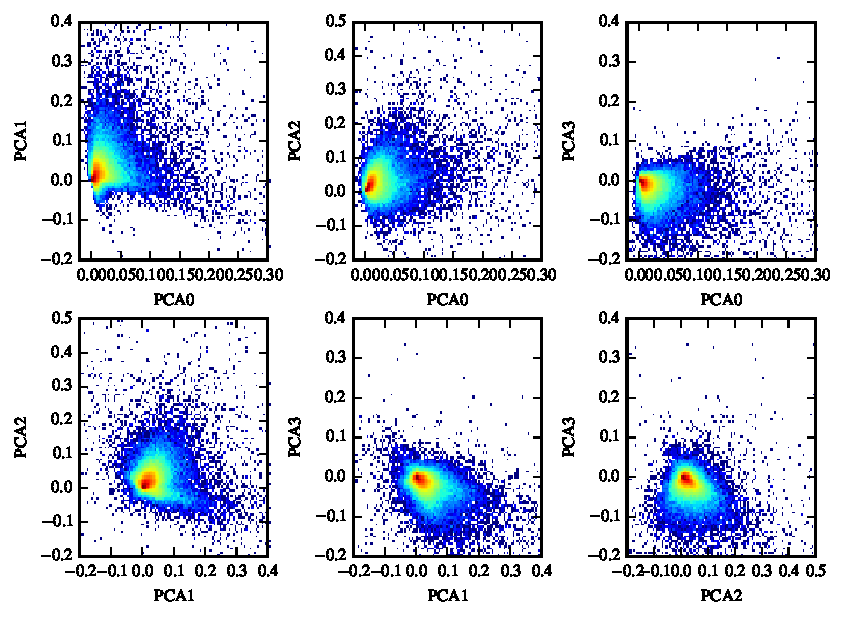
\includegraphics[width=5in]{figures/fig_sdss_pca.pdf}
\end{center}
 \vskip -0.20in
  \caption{\footnotesize PCA coefficients derived from $\approx
    100,000$ SDSS/DR7 quasars.  Color (red to blue) illustrates the
    number of sources at the plotted values.  Most of the variation in
    PCA0 derives from variations in the observed flux of these
    sources.  One does identify modest correlation between several
    pairs of the PCA components (e.g. PCA1 vs.\ PCA3).
  }\label{fig:sdss_pca}
\vskip -0.1in
\end{figure}

\subsection{BOSS/DR10}

We have analyzed approximately 100,000 quasars from BOSS/DR10, which
were used to study the Ly$\alpha$ forest by K.G. Lee ({\tt v2.1} of
his catalogs).  These quasars are almost exclusively at $z>2$, and as
with all BOSS spectra span the $\approx 3600-10,000$~\AA{} spectral
range. 

As in Section~\ref{sec:sdss} when analyzing the SDSS data, we derive
PCA coefficients from the BOSS spectra and find small variation in the
values.  Figure~\ref{fig:boss_pca_vs_i} shows the dependence of the
PCA values on $i$-band magnitude (which also correlates with
redshift).  As expected, {\tt PCA0}n shows the greatest correlation
with $i$-band magnitude.  We speculate that the dispersion in the PCA
values decreases with increasing magnitude owing to the poorer S/N of
the spectra.

\begin{figure}[h!]
  \vskip -0.1in
\begin{center}
  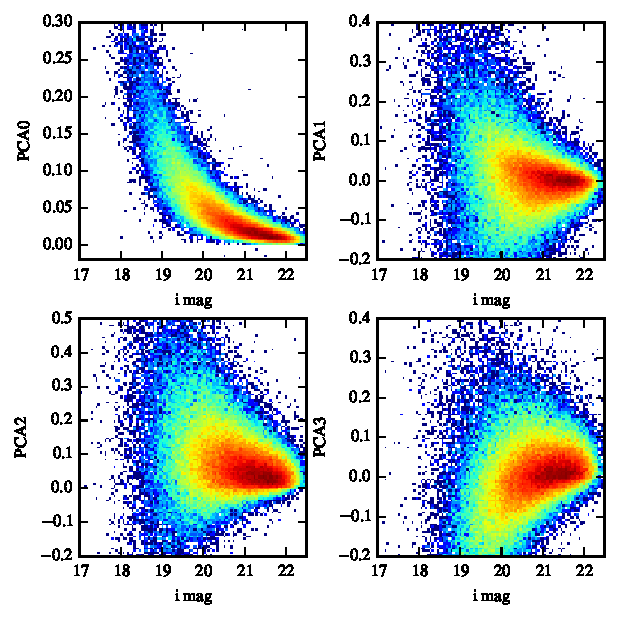
\includegraphics[width=5in]{figures/fig_boss_imag_vs_pca.pdf}
\end{center}
 \vskip -0.20in
  \caption{\footnotesize PCA coefficients of the BOSS/DR10 Ly$\alpha$
    sample as a function of $i$ magnitude.  As expected, {\tt PCA0}
    shows the greatest variation with observed quasar flux.  We
    suspect that the reduced dispersion in the PCA values with
    increasing magnitude is due to poorer S/N of those spectra, not a
    physical effect.  }\label{fig:boss_pca_vs_i}
\vskip -0.1in
\end{figure}


\section{QSO Templates}\label{sec:templ}

From the measured PCA values of the SDSS and BOSS samples, we proceed
to construct a set of 9,000 quasar templates as follows.  Note that we
use the SDSS models to construct templates at $z<2$ and the BOSS
spectra otherwise.

Stepping on a redshift interval of $\Delta z = 0.2$ and starting at
$z=0.2$, we generate {\tt N\_perz=500} quasar templates per $\Delta z$
interval to $z=4$.  For
these 500 templates we adopt the following approach:

\begin{enumerate}
\item Draw $z$ uniformly between the bounds of the interval.
\item For {\tt PCA0}, calculate the interval encompassing 95\%\ of the
  measured values.  These generally do not follow a Gaussian
  distribution.
\item For {\tt PCA1}, calculate the standard deviation.
\item Sample each PCA distribution uniformly over the 95\% confidence
  interval (i.e.\ $2 \sigma$ for {\tt PCA1-3}).
\item Generate a template from these random PCA values and the
  eigenvectors. 
\item Discard the template if the flux is negative in the rest-frame
  interval $900-5000$\AA.  This occurs approximately $5\%-10$\%\ of
  the time.
\item If $z \ge 2.4$, attenuate the flux shortward of $911.76$\AA\ in
  the rest-frame by a statistical estimate of the Lyman continuum (see
  below).
\item Convert to the observer frame and interpolate on a $\log_{10}$
  wavelength grid with $10$~km~s$^{-1}$ pixels starting at
  $3500$\AA\ and extending to $10,000$~\AA.
\end{enumerate}

For the Lyman continuum attenuation, we adopt the mean-free-path
$\lambda_{\rm MFP}$ estimates from Worseck et~al. (2014).
%\citet{worseck14a}
We then calculate the physical distance from the source $r_{\rm phys}$
with a standard $\Lambda$CDM cosmology ($\Omega_m = 0.3$), and then
attenuate the flux by $\exp(-r_{\rm phys} / \lambda_{\rm MFP})$. 

Figure~\ref{fig:gallery} shows a set of example templates.
The flux are in units of erg/s/cm$^2$/\AA\ and 
normalized to $10^{-17}$.

\begin{figure}[h!]
  \vskip -0.1in
\begin{center}
  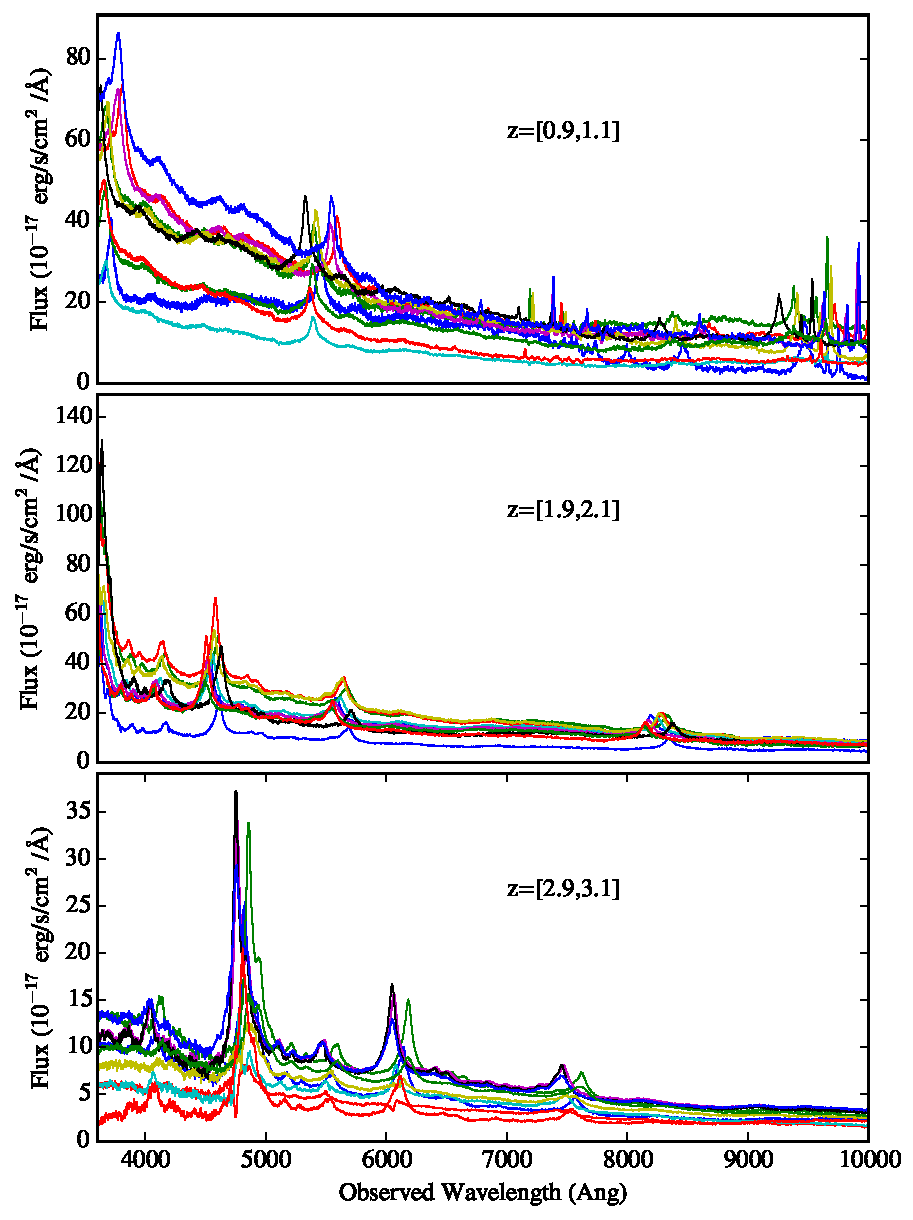
\includegraphics[width=5in]{figures/fig_desi_template_gallery.pdf}
\end{center}
 \vskip -0.20in
  \caption{\footnotesize Gallery of DESI quasar templates at $z \sim
    [1,2,3]$.  One observes a diversity of emission strengths,
    spectral slopes and IGM opacity.
}\label{fig:gallery}
\vskip -0.1in
\end{figure}


\section{Ancillary Information}

All of the codes for this analysis are in the DESI github repository
under py/qso\_template.  Here are the primary modules:

\begin{itemize}
\item {\tt fit\_boss\_qsos.py} -- Module for fitting the eigenvectors
  to the SDSS and BOSS spectra
\item {\tt run\_qso\_fits.py} -- Module for (simple) parallelization
  of the fitting
\item {\tt desi\_qso\_templ.py} -- Module for generating the DESI
  quasar templates
\item {\tt boss\_qsos\_figs.py} -- Module for generating figures from
  the various outputs.
\end{itemize}

Some of these codes draw on modules in the {\tt xastropy} and {\tt
  astropy} packages.

\vskip 0.2in


The templates can be found on NERSC in {\tt
  \$\{DESI\_ROOT\}/spectro/templates/qso\_templates/VERSION}, where
{\tt VERSION} is the template version number (currently v1.1).  The
template file itself, {\tt qso\_templates\_v1.1.fits} is a binary FITS
table with two extensions:

\begin{enumerate}
\item Extension~0: An [{\sc npixel}]$\times$[{\sc ntemplate}] flux
  array which contains {\sc ntemplate} spectra, each {\sc npixel}
  pixels long.
\item Extension~1: An [{\sc ntemplate}] data structure with the
  following metadata:
\begin{itemize}
\item{.{\sc TEMPLATEID} - unique template ID number (zero-indexed)}
\item{.{\sc Z} - redshift of the source}
\end{itemize}
\end{enumerate}

\section{Generating New Templates}\label{sec:new_templ}

Users may wish to generate templates beyond the v1.1 set.
The code has now been refactored to allow such activity.
Presently, the user generates a new FITS file containing 
the new set of templates.  The code also returns the specta
as simple numpy arrays.  

\begin{Verbatim}[commandchars=\\\{\}]
final_wave, final_spec, final_z = desi_qso_templates(outfil='test_random_set.fits', 
   N_perz=100, seed=12345)
\end{Verbatim}

The data necessary to run this
bit of code is currently here at NERSC: \\
{\tt /project/projectdirs/desi/spectro/templates/basis\_templates/v2.0/qso\_templates\_v2.0.fits}

\section{Future Improvements}\label{sec:future}

Future improvements to these templates may include (in no particular
order): 

\begin{itemize}
\item Masking of pixels in the PCA analysis.
\item Generate eigenvectors from the full and combined BOSS/SDSS datasets.
\item Apply the analysis to flux-corrected BOSS spectra.
\item Implementation of a stochastic Ly$\alpha$ forest.
\item Account for correlation between the PCA coefficients. 
\item Include BALs and other `unusual' quasars.
\end{itemize}

%\bibliographystyle{apj}
%\bibliography{/Users/ioannis/bibdesk/ioannis}
%\documentclass[11pt]{article}
\usepackage{epsfig}
\usepackage{amssymb}
\usepackage{fullpage}
\usepackage{color}
\usepackage{url}
\usepackage{natbib}
%\usepackage{emulateapj}
\usepackage{footnote}
\usepackage{deluxetable}
\usepackage{fancyvrb}

\newcommand{\aap}{A\&A}
\newcommand{\TODO}[1]{{\it \color{red} (#1)}}
\newcommand\codeHighlight[1]{\textcolor[rgb]{1,0,0}{\textbf{#1}}}

\begin{document}
\title{
DESI QSO Templates (v1.2)
}

\author{J. X. Prochaska (UCSC), J. Moustakas (Siena), S. Bailey
  (LBNL)}
\maketitle
\begin{center}

% Line below is modified automatically by svn, so don't edit it.
% Comment out the whole for final document
% (I first did : svn propset svn:keywords 'Id Author Date Rev' qso-templates.tex)
{\small SVN $ $Rev: 2833 $ $, $ $Date: 2014-12-22 07:28:33 -0800 (Mon, 22 Dec 2014) $ $, $ $Author: profx $ $ }
\end{center}

\abstract{ This technote documents the construction of the preliminary
  (v1.1) QSO templates for DESI.  It also describes how one may 
  generate new, random sets of QSO templates (on-the-fly) in desisim. }

\section{Introduction}

DESI will obtain high-resolution, observed-frame optical spectroscopy
of four broad classes of objects: quasars (QSOs), emission-line
galaxies (ELGs), luminous red galaxies (LRGs), and stars.  Reliable
spectral templates are critical for several key aspects of the
Project, including spectral simulations (constructing mock datasets),
optimization of targeting strategies, redshift fitting, spectral
classification, and other applications.

The general requirements on the spectral templates for all four
classes of objects are: (1) broad coverage of physical parameter
space; (2) wide wavelength coverage (minimum rest-frame
$\approx0.15-1~\mu$m spectral coverage); (3) high spectral
resolution (at least $\mathcal{R}\approx4500$); and (4) high
spectrophotometric fidelity.

This document describes the construction of the \emph{preliminary} QSO
templates for DESI.  These templates are generated from a PCA analysis
of SDSS/DR7 quasar spectra ($0.4<z<2$) and BOSS/DR10 quasar spectra
($z=2-4$), as described in Section~\ref{sec:sdssboss}.  We generated
500 templates per $\Delta z = 0.2$ interval from $z=0.4 - 4$,
uniformly sampling in redshift in each bin.  Further details on the
spectra are provided in Section~\ref{sec:templ}.

\section{SDSS/BOSS Spectroscopy}\label{sec:sdssboss}

\subsection{PCA Analysis}

The BOSS team has previously generated PCA eigenvectors from a sample
of approximately 450 quasars using the standard {\tt IDLSPEC2D}
algorithms.  The four eigenvectors are recorded in the file {\tt
  spEigenQSO-55732.fits}.  These spectra cover the rest-frame
450.2-10400\AA\ spectral range with a constant logarithmic dispersion
of $10^{-4}$~log$_{10}$~\AA{} (approximately $70$~km~s$^{-1}$ per
pixel).  We show these four eigenspectra in Figure~\ref{fig:eigen}.
One appreciates that most of the flux is in {\tt Eigen0} (as
expected), and that the eigenvectors are not physical representations
of actual quasars.  Nevertheless, we find these provide an excellent
basis for the observed spectra.

These eignevectors were fitted to observed SDSS and BOSS spectra using
standard least-squares (inverse variance weighted) fitting.  In this
analysis we do not use the spectral masks developed for BOSS, nor do
we develop our own masks (e.g.\ for known, bright sky lines).
However, we examined several tens of the fits by-eye to assess
performance and found generally good results.

\begin{figure}[h!]
  \vskip -0.1in
\begin{center}
  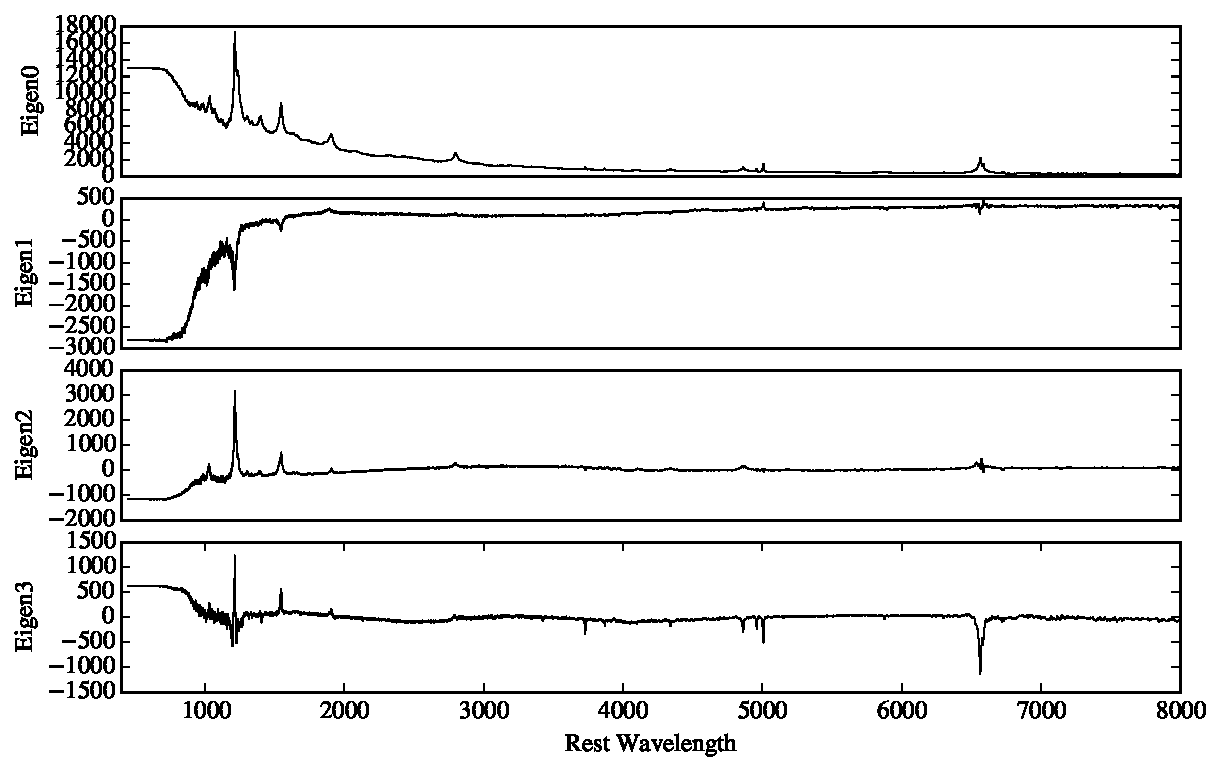
\includegraphics[width=5in]{figures/fig_boss_eigen.pdf}
\end{center}
 \vskip -0.20in
  \caption{\footnotesize 
    PCA eigenvectors drawn from the BOSS spectral package,
    specifically file spEigenQSO-55732.fits.  These span from $\approx
    450-10,400$\AA\ in the rest-frame.
 }\label{fig:eigen}
\vskip -0.1in
\end{figure}

\subsection{SDSS DR7}\label{sec:sdss}

We analyzed approximately 100,000 quasars drawn from the SDSS/DR7
quasar catalog, with spectra from the {\tt 1d\_26} extraction.  In our
adopted bins of $\Delta z = 0.2$, there are many thousands of spectra
per bin.  Unlike DESI (and BOSS), these data have a starting
wavelength of $\approx 3800$\AA.  Therefore, in the subsequent
analysis we assume a modest extrapolation of the solutions to bluer
wavelengths.  The models, however, appear well-behaved.

Figure~\ref{fig:sdss_pca} compares the distributions of the four PCA
coefficients derived for all of the SDSS spectra.  The variation in
the values is small, consistent with the small variation in quasar
spectral energy distributions (SEDs). Most of the variation in {\tt
  PCA0} derives from variations in the observed flux of these sources.
One does identify modest correlation between several pairs of the PCA
components (e.g. {\tt PCA1} vs.\ {\tt PCA3}).  When generating the
templates, however, we consider the PCA components independently. 

\begin{figure}[h!]
  \vskip -0.1in
\begin{center}
  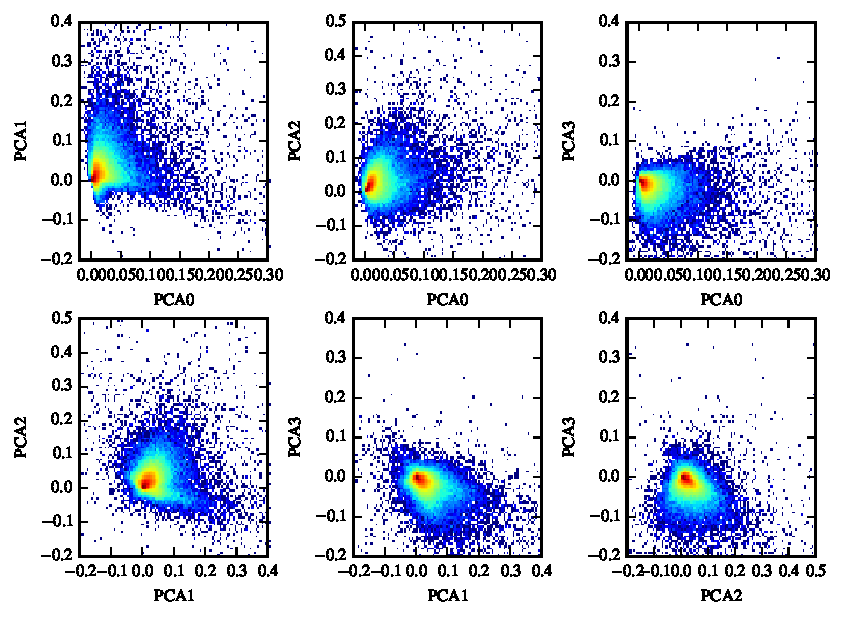
\includegraphics[width=5in]{figures/fig_sdss_pca.pdf}
\end{center}
 \vskip -0.20in
  \caption{\footnotesize PCA coefficients derived from $\approx
    100,000$ SDSS/DR7 quasars.  Color (red to blue) illustrates the
    number of sources at the plotted values.  Most of the variation in
    PCA0 derives from variations in the observed flux of these
    sources.  One does identify modest correlation between several
    pairs of the PCA components (e.g. PCA1 vs.\ PCA3).
  }\label{fig:sdss_pca}
\vskip -0.1in
\end{figure}

\subsection{BOSS/DR10}

We have analyzed approximately 100,000 quasars from BOSS/DR10, which
were used to study the Ly$\alpha$ forest by K.G. Lee ({\tt v2.1} of
his catalogs).  These quasars are almost exclusively at $z>2$, and as
with all BOSS spectra span the $\approx 3600-10,000$~\AA{} spectral
range. 

As in Section~\ref{sec:sdss} when analyzing the SDSS data, we derive
PCA coefficients from the BOSS spectra and find small variation in the
values.  Figure~\ref{fig:boss_pca_vs_i} shows the dependence of the
PCA values on $i$-band magnitude (which also correlates with
redshift).  As expected, {\tt PCA0}n shows the greatest correlation
with $i$-band magnitude.  We speculate that the dispersion in the PCA
values decreases with increasing magnitude owing to the poorer S/N of
the spectra.

\begin{figure}[h!]
  \vskip -0.1in
\begin{center}
  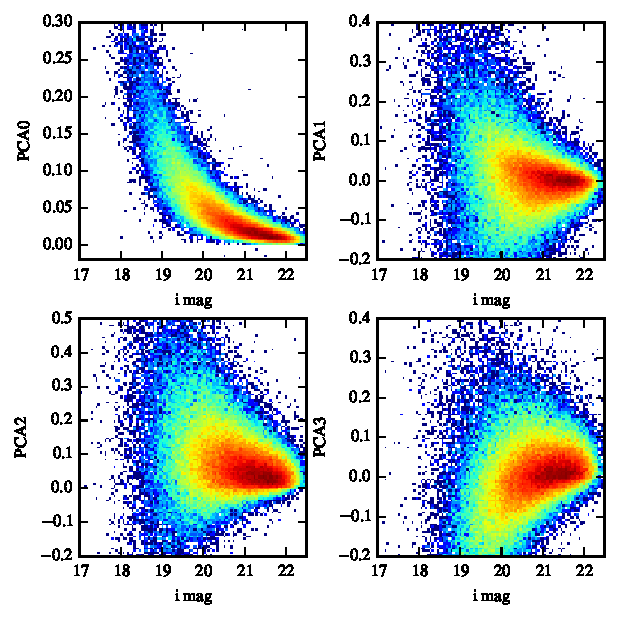
\includegraphics[width=5in]{figures/fig_boss_imag_vs_pca.pdf}
\end{center}
 \vskip -0.20in
  \caption{\footnotesize PCA coefficients of the BOSS/DR10 Ly$\alpha$
    sample as a function of $i$ magnitude.  As expected, {\tt PCA0}
    shows the greatest variation with observed quasar flux.  We
    suspect that the reduced dispersion in the PCA values with
    increasing magnitude is due to poorer S/N of those spectra, not a
    physical effect.  }\label{fig:boss_pca_vs_i}
\vskip -0.1in
\end{figure}


\section{QSO Templates}\label{sec:templ}

From the measured PCA values of the SDSS and BOSS samples, we proceed
to construct a set of 9,000 quasar templates as follows.  Note that we
use the SDSS models to construct templates at $z<2$ and the BOSS
spectra otherwise.

Stepping on a redshift interval of $\Delta z = 0.2$ and starting at
$z=0.2$, we generate {\tt N\_perz=500} quasar templates per $\Delta z$
interval to $z=4$.  For
these 500 templates we adopt the following approach:

\begin{enumerate}
\item Draw $z$ uniformly between the bounds of the interval.
\item For {\tt PCA0}, calculate the interval encompassing 95\%\ of the
  measured values.  These generally do not follow a Gaussian
  distribution.
\item For {\tt PCA1}, calculate the standard deviation.
\item Sample each PCA distribution uniformly over the 95\% confidence
  interval (i.e.\ $2 \sigma$ for {\tt PCA1-3}).
\item Generate a template from these random PCA values and the
  eigenvectors. 
\item Discard the template if the flux is negative in the rest-frame
  interval $900-5000$\AA.  This occurs approximately $5\%-10$\%\ of
  the time.
\item If $z \ge 2.4$, attenuate the flux shortward of $911.76$\AA\ in
  the rest-frame by a statistical estimate of the Lyman continuum (see
  below).
\item Convert to the observer frame and interpolate on a $\log_{10}$
  wavelength grid with $10$~km~s$^{-1}$ pixels starting at
  $3500$\AA\ and extending to $10,000$~\AA.
\end{enumerate}

For the Lyman continuum attenuation, we adopt the mean-free-path
$\lambda_{\rm MFP}$ estimates from Worseck et~al. (2014).
%\citet{worseck14a}
We then calculate the physical distance from the source $r_{\rm phys}$
with a standard $\Lambda$CDM cosmology ($\Omega_m = 0.3$), and then
attenuate the flux by $\exp(-r_{\rm phys} / \lambda_{\rm MFP})$. 

Figure~\ref{fig:gallery} shows a set of example templates.
The flux are in units of erg/s/cm$^2$/\AA\ and 
normalized to $10^{-17}$.

\begin{figure}[h!]
  \vskip -0.1in
\begin{center}
  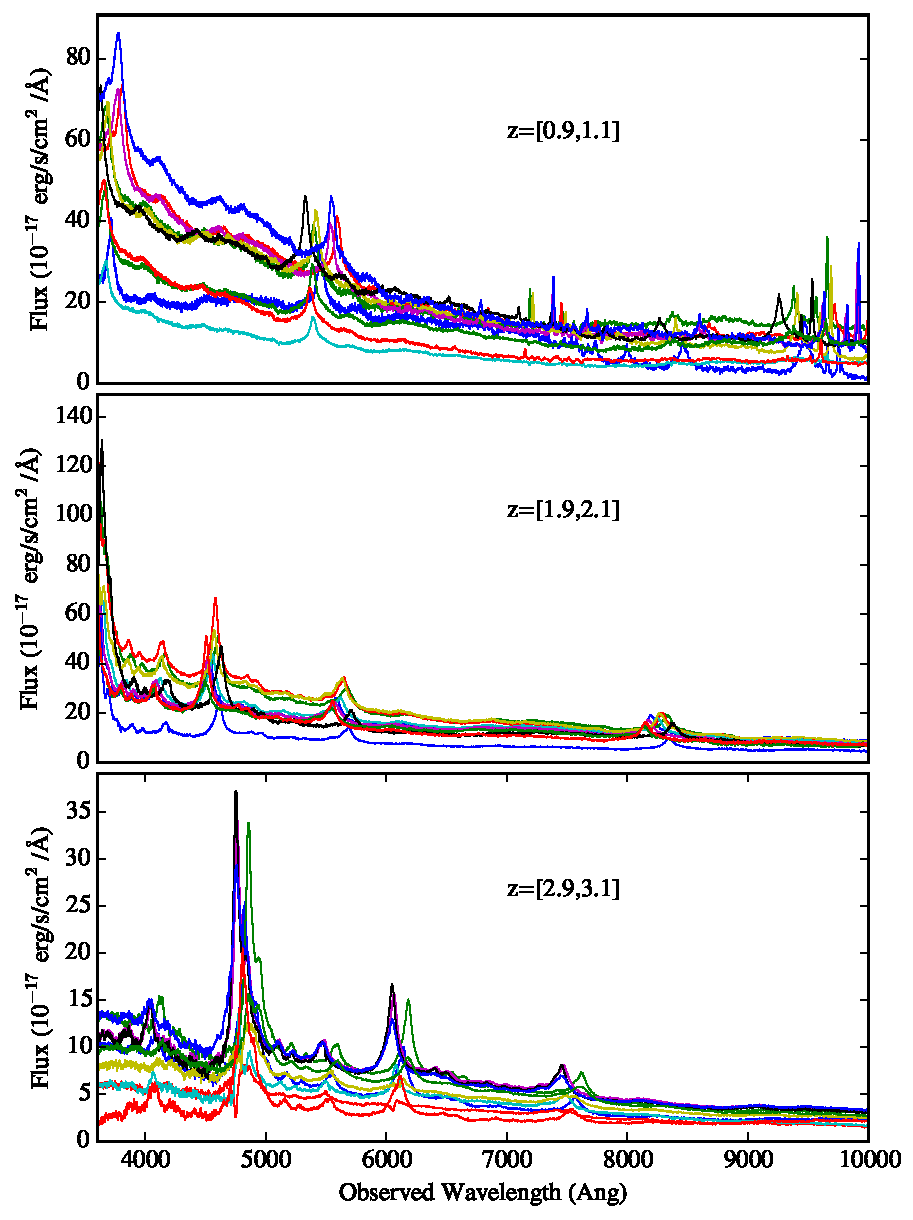
\includegraphics[width=5in]{figures/fig_desi_template_gallery.pdf}
\end{center}
 \vskip -0.20in
  \caption{\footnotesize Gallery of DESI quasar templates at $z \sim
    [1,2,3]$.  One observes a diversity of emission strengths,
    spectral slopes and IGM opacity.
}\label{fig:gallery}
\vskip -0.1in
\end{figure}


\section{Ancillary Information}

All of the codes for this analysis are in the DESI github repository
under py/qso\_template.  Here are the primary modules:

\begin{itemize}
\item {\tt fit\_boss\_qsos.py} -- Module for fitting the eigenvectors
  to the SDSS and BOSS spectra
\item {\tt run\_qso\_fits.py} -- Module for (simple) parallelization
  of the fitting
\item {\tt desi\_qso\_templ.py} -- Module for generating the DESI
  quasar templates
\item {\tt boss\_qsos\_figs.py} -- Module for generating figures from
  the various outputs.
\end{itemize}

Some of these codes draw on modules in the {\tt xastropy} and {\tt
  astropy} packages.

\vskip 0.2in


The templates can be found on NERSC in {\tt
  \$\{DESI\_ROOT\}/spectro/templates/qso\_templates/VERSION}, where
{\tt VERSION} is the template version number (currently v1.1).  The
template file itself, {\tt qso\_templates\_v1.1.fits} is a binary FITS
table with two extensions:

\begin{enumerate}
\item Extension~0: An [{\sc npixel}]$\times$[{\sc ntemplate}] flux
  array which contains {\sc ntemplate} spectra, each {\sc npixel}
  pixels long.
\item Extension~1: An [{\sc ntemplate}] data structure with the
  following metadata:
\begin{itemize}
\item{.{\sc TEMPLATEID} - unique template ID number (zero-indexed)}
\item{.{\sc Z} - redshift of the source}
\end{itemize}
\end{enumerate}

\section{Generating New Templates}\label{sec:new_templ}

Users may wish to generate templates beyond the v1.1 set.
The code has now been refactored to allow such activity.
Presently, the user generates a new FITS file containing 
the new set of templates.  The code also returns the specta
as simple numpy arrays.  

\begin{Verbatim}[commandchars=\\\{\}]
final_wave, final_spec, final_z = desi_qso_templates(outfil='test_random_set.fits', 
   N_perz=100, seed=12345)
\end{Verbatim}

The data necessary to run this
bit of code is currently here at NERSC: \\
{\tt /project/projectdirs/desi/spectro/templates/basis\_templates/v2.0/qso\_templates\_v2.0.fits}

\section{Future Improvements}\label{sec:future}

Future improvements to these templates may include (in no particular
order): 

\begin{itemize}
\item Masking of pixels in the PCA analysis.
\item Generate eigenvectors from the full and combined BOSS/SDSS datasets.
\item Apply the analysis to flux-corrected BOSS spectra.
\item Implementation of a stochastic Ly$\alpha$ forest.
\item Account for correlation between the PCA coefficients. 
\item Include BALs and other `unusual' quasars.
\end{itemize}

%\bibliographystyle{apj}
%\bibliography{/Users/ioannis/bibdesk/ioannis}
%\input{qso-templates.bbl}

\end{document}


\end{document}


\end{document}


\end{document}
